\documentclass[a4paper,10pt]{article}
\usepackage[utf8]{inputenc}
\usepackage{authblk}
\usepackage{tabularx}
\usepackage{url}
\usepackage{graphicx}
\graphicspath{{images/}}
\usepackage{caption}

\title{SuperMat: Construction of a linked annotated dataset from superconductors-related literature}
% \title{SuperMat: Construction of a linked annotated dataset for superconductors material discovery}
% \title{SuperMat: Construction of a linked annotated dataset to support superconductors material research}

\author[1]{Luca Foppiano\thanks{FOPPIANO.Luca@nims.go.jp}}
\author[1]{Sae Dieb}
\author[1]{Akira Suzuki}
\author[2]{Pedro Baptista de Castro}
\author[2]{Suguru Iwasaki}
\author[2]{Yan Meng}
\author[2]{Terashima Kensei}
\author[2]{Yoshihiko Takano}
\author[1]{Masashi Ishii\thanks{ISHII.Masashi@nims.go.jp}}

\affil[1]{Material Database Group, MaDIS, NIMS, Japan}
\affil[2]{Nano Frontier Superconducting Materials Group, MANA, NIMS}

\begin{document}

\maketitle

\begin{abstract}
% background and related work 
% material science 
% our work 

%The creation of large collaborative projects such as the Materials Genome Initiative~\cite{material_genome_initiative}, contributed to accelerate the change, however the amount of structured data represent a negligible part of the potentially available information.

%At the moment, the only available database for superconducting material discovery is Supercon, which is old, small (only 30000 entries) and outdated. There is needs of modernising or rebuilding the current manual process, which cannot keep-up with the current publication rate. 
% We are currently working on a collaborative project to implement a system for mining information from superconductors-related literature using different approaches of machine learning and rule-based. 

% We annotated entities such as materials, classes, measurement methods, and properties such as superconducting critical temperature values and expressions, and critical pressure. We linked materials with critical temperature, pressures, and measurement methods. 


% importance of text and data mining in material research (max 2 sentences) 
In materials science, abundant publications are available as knowledge source. However, information are presented mainly as text, which cannot be used as machine-readable media.
% information provided as text in a non-standardised and unstructured form, is 
The development of Text and data mining (TDM) processes is necessary to exploit this prosperity of information in many ways. Scientists can benefit this information overloading, for example, by semantic information retrieval, or by automatic document synthesis. 
In material discovery, breakthrough can be achieved by providing potential candidate materials in respect of certain properties, for example superconductivity or magnetic capabilities. 
%to accelerate toward breakthrough by exploiting the vast knowledge hidden in scientific literature. 

% The National Institute for Materials Science (NIMS) has been investing in establishing TDM processes to support material discovery. 
% manually constructing several databases to support materials research, and SuperCon\footnote{\url{http://supercon.nims.go.jp}} was a hopeful data source for superconductor domain. 
% Importance of superconducting material research 
Superconductors materials are already used as components in many applications~\cite{Hoshino2015InnovativeLR, Kizu2010ConstructionOT, Cardani2017NewAO, THOMAS201659},  and the research is still active~\cite{Drozdov_2019} but requires effort to fully switch to a data-driven approach\cite{Hamlin2019SuperconductivityNR}. 

% other attempts 
% However, only few attempts of applying TDM in materials literature have been described by \cite{Dieb2011ConstructionOT}, \cite{court2018auto} and \cite{kononova_text-mined_2019}. 

%% What we did 
We created a new dataset to provide solid foundations for establishing TDM processes for researchers of the superconductors domain and beyond: SuperMat (Superconductor Materials). Supermat is an annotated dataset of linked data of materials, properties and conditions from scientific literature. 

% How we did it 
This work has been carried out as collaborative project between computers and materials scientists and includes the documentation of the process and the annotation guidelines.
Our work is articulated over an iterative process composed by 4 main tasks: (1) relevant information selection, (2) tag-set and relationship design, (3) annotation rules definitions, and (4) validation by domain experts.
The dataset, composed by 114 articles and 9966 entities  (or which, 4000 unique), contains annotations of materials, samples, classes, properties (superconducting critical temperature, measurement method), and conditions (applied pressure). 
Relationships between certain entities is also annotated:  superconducting critical temperature (\textit{Tc}) with parametric conditions such as pressure values, and the used methods of measurements, when specified.

% What we found out 
We measured the Inter Annotation Agreement (IAA) between different classes of technicians (Computer Scientist, Material Scientists and Students) compared with domain experts. We reached a satisfying average agreement with domain experts. We noticed that students of materials science were challenged the most, indicating that the knowledge of only physics is not enough to successfully carry out the annotation task.

% What we conclude
SuperMat can be used to develop TDM processes for many complementary tasks such as information retrieval, document synthesis, information clustering. 
Our methodology and guidelines provides a trail that can be followed as a general approach in other domains. 
We utilised this dataset to train a sequence labelling system, which was then applied to semantically enhance a search engine for scientific documents and a document classification system using superconductors-related classes. 

    
\end{abstract}

\newpage

\section{Background and summary}
% Introduction, why text is important for scientific knowledge? 
The vast majority of scientific knowledge is available, with overwhelming abundance~\cite{Grigas2017JustGI, Khabsa2014TheNO, OrduaMalea2015MethodsFE, Bjrk2009ScientificJP}, through published papers and articles. 
However, most of the information are presented as text, which is an arbitrary and unstructured form of communication, difficult to be used as machine readable media. 
% TDM and its importance - next sentence needs to link the a) abundance, and b) unstructured with the end result (structured data) -> TDM For the win... 

The computer-assisted process for identifying and collecting information from scientific literature, also referred to as Text and Data Mining (TDM), is a supportive asset for scientific research. 
In the past decades, TDM processes have evolved their ability to perform automatic document processing such as document synthesis, information retrieval and entity extraction. 

%The establishment of Text and Data Mining (TDM) processes is an unavoidable step to bridge information collected from scientific literature toward data-driven discovery. 

Looking at the scientific literature, several corpora has been created in other domains, to mention the most important: BioCreative IV CHEMDNER corpus~\cite{Krallinger2015TheCC} in chemistry, and Genia~\cite{Kim2003GENIAC} and GENETAG~\cite{Tanabe2005GENETAGAT, Ohta2009IncorporatingGA} in biology. In material science, we can mention NATDEV~\cite{Dieb2016} to support research of nanocrystal devices and, a material-synthesis corpus, for extracting systhesis recipes~\cite{kononova_text-mined_2019}. 

% Practical example in biology 
In biology, TDM has been applied in information extraction to identify agents interaction (e.g. bacteria, virus, genes, proteins)~\cite{10.1371/journal.pone.0004554, Krallinger2010, Krallinger2009ExtractionOH} or to support the research against serious diseases, like cancer~\cite{Krasnitz2019CancerB}. 
Chemical compounds name disambiguation, synthesis extraction and retrieval are other examples of TDM applications in chemistry~\cite{Hawizy2011ChemicalTaggerAT}.

% Dieb: Why collecting information from text is useful for material science? 
Materials science has been lagging behind. In many areas, materials scientists relies on theoretical approaches, such as Density Functional Theory (DFT) or ab-initio calculations, often based on manually extracted data. 
The adoption of data-driven computation (today called Materials Informatics (MI)) had been facing several challenges: lack of data standard, difficult to understanding the practical data-driven applicability, wide variety of conflicting stack-holders, and missing incentives to contributed to large collaborative initiatives~\cite{Hill2016MaterialsSW}. 

%% Add a sentence that state how TDM processes can help research in material science 
Like in other disciplines, materials scientists can benefit from TDM processes in many ways. 
For example, reducing the time needed looking for information by providing semantically enriched search engines able to accept very precise query~\cite{Liu2019SurfaceMR}. 
Secondly, and equally important, is to ease off the burden to collect structured data. Automatic process for dataset extraction will enable scientists to focus and leverage computing power for finding deeper relationships between information potentially unrelated.
All these process cannot be easily established without basic resources like dictionaries, lexicons, datasets. Materials-related or physical quantities dictionaries or publication-based datasets with annotated entities to mention some examples. 

%For example, to help researchers retrieving information based on very granular search queries, to extract structured datasets automatically, or to aggregate information by semantic similarity. suitable to be the input data of deep analysis processes   or properties prediction (curie temperature, magnetocaloric temperature, etc...).

% Superconductors domain
%   - concrete example of superconducting case -> which properties or information can be useful for superconducting material scientists? [Suzuki/Terashima/Pedro]

High-temperature superconductors have many promising applications. They are already present as specific components of quantum computers and medical instruments, or to support efficient energy production~\cite{Hoshino2015InnovativeLR, Kizu2010ConstructionOT, Cardani2017NewAO}. 
However, to discover a new superconductor is very difficult, it is said that only 3\% of candidate materials is actually a superconductor~\cite{Konno2018DeepLO}.
The National Institute for Materials Science (NIMS) has been manually constructing several databases to support materials research, and SuperCon\footnote{\url{http://supercon.nims.go.jp}} was a hopeful data source for superconductor domain. 
%%[How Supercon is supposed support material research]
Its data has been used to develop systems for predicting superconducting critical temperature (\textit{Tc})~\cite{stanev2017machine}. Potentially, it can leverage processes for designing new materials with higher \textit{Tc}, ideally up to room temperature~\cite{Hamlin2019SuperconductivityNR}. One way to support superconductors research is to increase and enrich the available data (Supercon, for example).
%(NOTE this is just an example on how a database can support material research)
% We need to go back to how we can support superconductors research 


%unexplored terrain. 

% There are no records of corpora constructed in the superconductors domain. 

In this paper, we present our inter-disciplinary work for creating a linked dataset for superconductor material data: SuperMat (Superconductors Materials). We created a dataset with linked information which can support the development of new TDM processes starting from the superconductors domain, but potentially extensible to other domains within materials science. 

%[Summarise the approach]
We collected papers related to research in superconductivity from different sources and publishers.  
We designed the tag sets by combining the examination of the scientific articles and the guidance based on the domain experts experience and needs. 
We defined an iterative annotation process which was composed by four steps: a) annotation guideline construction, b) annotation of relevant mentions, c) validation of the annotated data from domain experts, and d) review. This process allowed us improve simultaneously  both annotations and guidelines at every iteration. 

As a result, we produced a dataset composed by 114 articles, with 9966 entities (of which, about 4000 unique entities value). They were annotated using six classes, described in details in section \ref{sec:method}: material, class, critical temperature expressions, critical temperature value, critical pressure value and measurement method.
We added a layer of links between entities, of three types: 1) \textit{material-tc} linking materials and their respective superconducting critical temperature \textit{Tc}. 
2) \textit{tc-pressure} connecting \textit{Tc} and the applied pressure at which it was obtained, and 3) \textit{tc-me\_method} between the critical temperature with the method used to obtain the measurement. 
The superconducting critical temperature is susceptible to conditions such as magnetic field or pressure. 

[Should we add a sentence describing the number of annotators and their background? Should we mentioned IAA?]

% usage of dataset
SuperMat can be used to develop TDM processes for achieving many complementary tasks: 
1) creation of automatic system for dataset creation, 
2) articles classification, 
3) named entity extraction, for example to construct dictionaries of terms, 
4) clustering and document synthesis ,
5) training of Machine Learning (ML) algorithms,
6) evaluation of rules-based or ML-based algorithms, and 
7) development of downstream processes, such as material name parser, or quantities normalisation.

This dataset is potentially suitable to be applied to other materials science domains, such as magnetocaloric, spintronic related research. 
%In the future we plan to extend the information provided (e.g. including magnetic fields) and to complement this dataset with articles from other domains. 

The paper is structured as follows: after the introduction, we discuss the methodology used to obtain the data and to produce the final result. Then we describe the information and the validation of the data contained in the dataset. Finally, we provide example of applications, usability and availability information. 

% [END]
% -- 

% [OLD] Data-driven science has become as the fourth dimension in scientific exploration, after experimentation, theory and simulation~\cite{doi:10.1063/1.4944682}.


% [OLD] The emergence of Machine Learning (ML), a sub-field of Artificial Intelligence (AI), followed by a growing infrastructure of tools for generating, testing, and refining scientific models give us some hope. Such approach allow to address complex problems which conventional techniques cannot solve efficiently. 

% Introduce the importance of high-quality training data 
% [OLD] On the other hand the development of statistical models require a solid base where to build more complex systems. Low quality or incorrect data, will propagate and exponentially impact on the out result. One of the dogma of text processing is "Garbage in, Garbage out", therefore is foremost important to reduce at minimum the "Garbage in" by having high quality data. 


% to be rephrased
%Contrary to what might seem like the conventional machine learning mantra, throwing more data at the problem is not always the solution. Instead, the quality and domain-specificity of the corpus determine its effectiveness for domain-specific tasks.

% In the field of superconductors materials, the manual data collection used to populate SuperCon\footnote{\url{http://supercon.nims.go.jp}} cannot cope with the massive fresh information from the increasing number of articles published every year. In addition, the current process cannot easily scale infinitely, for physical and economical constraints. 
%- 

%-

% A project is currently ongoing, and aims to develop a system for automatic superconductors database creation. From large quantities of superconductors{-}related articles, it aims to extract, automatically, superconductors material and their relative properties~\footcite{foppiano2019proposal}. 

% The dataset provides scientific text annotated with entities and relationship information (links). The entities are identified among 6 classes (or labels) as summarised in Figure~\ref{fig:classes_frequency} and linked using relationships \texttt{material-tc} and \texttt{tc-pressure} (Table~~\ref{tbl:summary-links}). 

% This corpus is designed for training sequence labelling statistical models and can be utilised for developing domain-specific systems for entity extraction, entity-relationship and clustering. 

%Recently, however, thanks to large collaborative projects such as the Material Genome Initiative~\cite{material_genome_initiative}, the data-driven approach gained popularity. 
%The term Materials Informatic (MI) is used for defining the sub-domain dedicated to computational discovery. 
%Unfortunately, the number of structured material data still represents a negligible part of the available knowledge. 
%Most of them, such as AFlow~\cite{CURTAROLO2012218}, Polynfo~\cite{polynfo}, the Pauling File~\cite{Blokhin2018ThePF_paulingFile} have been manually constructed and curated over decades. 
%Manual curation, that in many sub-domain is culturally believed as the safest approach to ensure quality, is becoming both technically and economically unsustainable. 
%The creation of automatic TDM processes for database creation is therefore a necessary milestone to ensure the availability of large structured databases. 


%to both unstructured (freely available scientific articles of Medline or PubMed Central) and structured (experimental data, patient clinical information) resources [ADD CITATION] 
%One example is the largest collaborative biological project, the Human Genome Project [TODO: add citation] was started back in 1984 and completed in 2003. 


%Today, unfortunately, this process cannot cope with the number of new yearly publications. 
%The development of an automatic system is therefore necessary. [How to introduce the needs of the data? the egg or the chicken ]


%[TODO: introduce the use of Machine Learning]
%Machine Learning provides higher tolerance to noise and faster generalisation capabilities than classical rule-based approaches. Even though rule-based approaches do not need training data, they also require a dataset for evaluate the performances. In addition, writing rules from scratch, can lead to [REWRITE trasversal problem], meaning that one rule can fix one problem and break another. 

%   - needs of information in superconductors
%   - the available databases are a) old, b) small, c) manually constructed -> outdated
%   - automatic extraction is required 
% Dieb: Why the construction of the corpus is useful? 
%   - what is the related work? mention other corpora 
%   - need of training data for creating the model / system 

\label{sec:method}
\section{Method}
\subsection{Content acquisition}
Our content is composed by scientific articles. Mention the input data 

We collected the content from several sources. (a) the Open Access version of articles referenced in the SuperCon database records. (b) Articles of interests according with domain-experts research topics. (c) Articles from the arXiv's “Condensed matter” category\footnote{\url{https://arxiv.org/archive/cond-mat}} obtained, by searching with keywords such as 'superconductor', 'critical temperature' and 'superconductivity'.

The Open Access version was obtained by using the service biblio-glutton lookup\footnote{\url{https://github.com/kermitt2/biblio-glutton}}, a Lookup service for bibliographic data which combine the database from Crossref\footnote{\url{https://www.crossref.org/}} and the service unPaywall\footnote{\url{http://unpaywall.org}}. 

\begin{figure}[h]
    \centering
    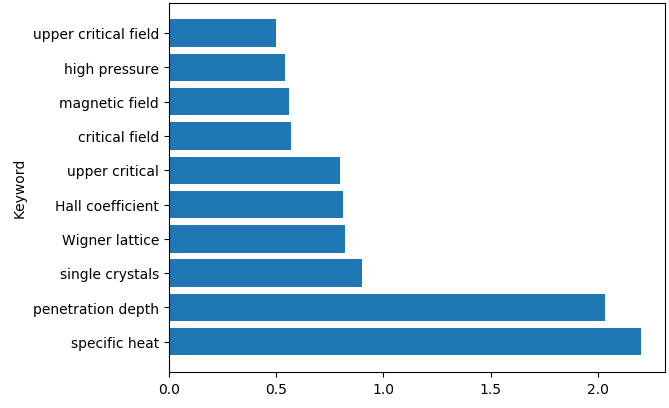
\includegraphics[width=\linewidth]{keyword-top10-body-distribution}
    \captionof{figure}{Distribution by keyword extracted from the articles body. }
    \label{fig:keyword-top10-body}
\end{figure}

\begin{figure}[h]
    \centering
    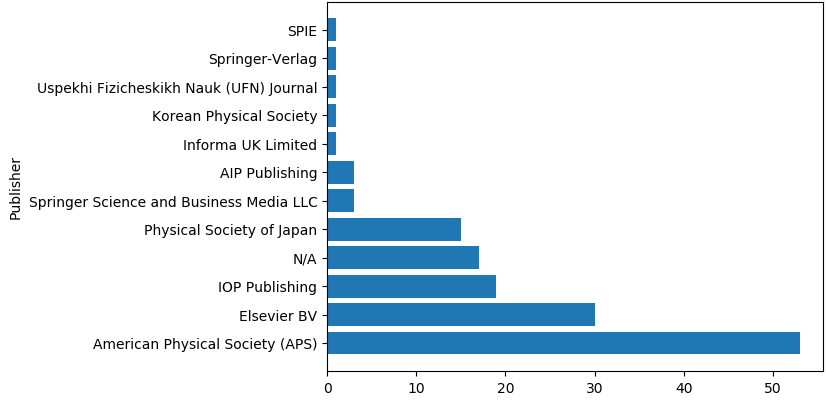
\includegraphics[width=\linewidth]{paper-by-publishers}
    \captionof{figure}{Distribution by publisher extracted from the articles body. }
    \label{fig:keyword-top10-body}
\end{figure}

\begin{figure}[h]
    \centering
    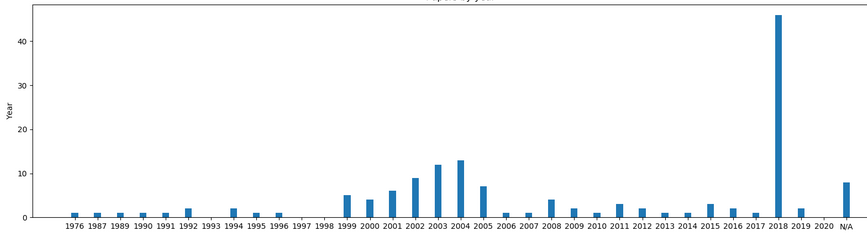
\includegraphics[width=\linewidth]{supermat-distribution-by-year}
    \captionof{figure}{Distribution by publisher extracted from the articles body. }
    \label{fig:keyword-top10-body}
\end{figure}

\begin{figure}[h]
    \centering
    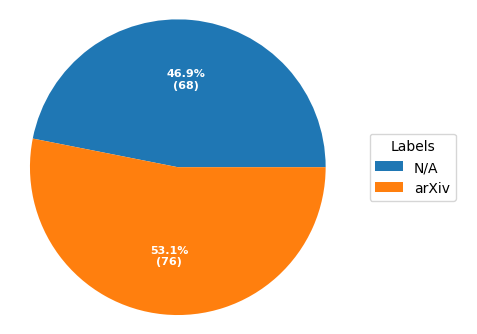
\includegraphics[width=\linewidth]{pie-arxiv-papers.png}
    \captionof{figure}{Rate of arXiv papers.}
    \label{fig:keyword-top10-body}
\end{figure}

The corpus was obtained starting from PDF because 
1. PDF is the most common format used for scientific article
2. the availablility of the XML version was subject to tight restrictions 
3. The text extracted from XML has two main problems: 
 - it is perceived to be cleaner, although error are still present, and their impact is higher, as it is assumed they are not present 
 - the XML is provided in a very ehterogeneus way, 
 - not all the papers in XML contain fulltext 
 - PDF extracted data is roughly more noisy, which could contribute to create more robust systems 

The corpus was collected in batches, which are simpler to manage, with the growing dimension. 

\subsection{Tag-set design}
The tag-set represent the labels and relative information that we want to capture. We discussed with domain-experts, the end clients of our system, what are the relevant information and entities they are interested in, in order of importance. We wanted to find the optimal trade-off that could keep the system simpler, yet providing all main needed information for domain experts. 

As a result, we compiled a summary table (Table \ref{table:summary-entities-superconductor}) of relevant entities, in order of importance for domain experts [TODO: waiting for an prioritised version of this table from Takano Gr. ].

\begin{table}[h!]
    \centering
    \begin{tabular}{ | m{5em} | m{8cm}| m{5em} | } 
    \hline
        Name & Description & type \\ [0.5ex] 
    \hline\hline
        T\textsubscript{c} & Superconducting critical Temperature & result\\ 
    \hline
        T\textsubscript{onset} & Temperature at which the electrical resistance starts to decrease sharply & result\\
    \hline 
        T\textsubscript{offset} & Temperature at which zero resistance starts to appear & result\\ 
    \hline
        P & Superconducting critical pressure & condition\\
    \hline
        Material & Material composing the sample & sample \\
    \hline  
        Substrate & Material layers composing the sample & sample\\
    \hline
        Crystal structure space group & Crystal configuration (single crystal, poly-crystal) & sample \\
    \hline 
        Preparation shape & wire, powder, crystal, thin film & sample\\
    \hline 
        Measurement method & Method used for measuring the superconducting critical temperature (theoretical/calculation, electrical resistivity, magnetic susceptibility and specific heat) & measurement\\
    \hline
        H\textsubscript{c1} & Lower Critical field & condition\\ 
    \hline
        H\textsubscript{c2} & Higher Critical field & condition\\ 
    \hline
        I\textsubscript{c} & Critical current & condition\\
    \hline
        J\textsubscript{c} & Critical current density & condition\\ 
    \hline
        H\textsubscript{ivr} & Irreversibly field & condition\\
    \hline    
        Fabrication process & process used to fabricate the sample & sample\\
    \hline    
    \end{tabular}
    \caption{Summary of the relevant entities in superconductor research papers}
    \label{table:summary-entities-superconductor}
\end{table}

We decided to focus on extracting information from text as this first initial stage. Table or plot extraction can be run as separate parallel projects.  

\textbf{Class} (tag: \texttt{<class>}) represent a group of materials having similar characteristics or common strategic compounds that define their nature are represented by classes. 

The material’s class in the superconductors-related domain does not follow a strict definition. Some of the superconductors classes can be inferred from the composition of the materials such as cuprates, iron-based, etc. There is a secondary level classification, which is more arbitrary and domain experts learn with experience.

\textbf{Material} (tag: \texttt{<material>}) identifies a name of one or more materials, a sample of a material, a doped sample and include additional information such as shape, fabrication when they are provided  ajointed to the material name. 

\textbf{Superconducting critical temperature expression} (tag: \texttt{<tc>}) represents expressions providing information about the phenomenon of superconductivity which is related to a critical temperature. This includes also explicit mention to the presence (e.g. /textit{This material is a superconductor}) or absence (e.g. /textit{This material is not a superconductor}).

\textbf{Superconducting critical temperature value} (tag: \texttt{<tcValue>}) represent the value of the superconducting critical temperature, Tc. Other temperatures (fabrication conditions, etc.) should not be annotated.

\textbf{Applied pressure} (tag: \texttt{<pressure>}) when superconductivity is measured. The superconductor critical temperature can be triggered by different conditions, one of the most studied is, in fact, the application of pressure. 

\textbf{Measurement method} (tag: \texttt{<me\_method>}) sndicates the techniques used to measure or calculate the presence of superconductivity. This includes also the study of temperature/resistivity, temperature/magnetic field graphs, not necessarily related to superconductivity.

\subsection{Annotation process}
\label{sec:annotation-process}

\subsubsection{Transformation of data}
\subsubsection{Annotation guidelines}
\subsubsection{Preliminary annotation}
\subsubsection{Machine-based annotated data}
\subsubsection{Annotation process}
\subsubsection{Validation from Domain experts}
\subsubsection{Inter Annotation Agreement / Review}

We describe the annotation process as a variation of the MATTER approach: Model, Annotate, Train, Test, Evaluate, and Revise, which was initially described by [ADD CITATION]. 

Our system uses already established open-source libraries which are providing already several functionalities which can simplifying our workflow. Our workflow consists in the following steps: Pre-annotate, Correct annotation, Validate, Train/Test/Evaluate, Revise. 

We are under the assumption of having a system implementing some sort of recognition (a machine learning model trained with one document or a rule-based approach) to bootstrap the process. 

The data is pre-annotated, then annotators can correct these annotations. Once a document is completed, it is validated by domain experts, which are checking the document again. This process brings two benefits: reduce distraction errors, and validate the annotation from the domain point of view. 
[TODO: add schema summarising this process]

The pre-annotation 

The correction


\section{Data Record}
Description of the analysis of the dataset 

This section should be used to explain each data record associated with this work, including the repository where this information is stored, and to provide an overview of the data files and their formats. Each external data record should be cited using our data citation format format.



\section{Applications}
How the corpus can be used

\section{Technical Validation} 
This section should present any experiments or analyses that are needed to support the technical quality of the dataset. This section may be supported by figures and tables, as needed.

Write about the results of the comparison between 
- CS vs DE 
- MS vs DE
- Kubokawa-san / Meng-san vs DE? 

%\section{Data Usage} 
%Describe how the data is provided XML, JSON... 

\section{Code Availability}
where, how the data will be distributed 

Github? MDR, Nomad? 


\section{Conclusion}
Conclusions and future work 

% IAA
% We have analysed the process and the evolution of the agreement during our process and how this can be used to understand when certain constraints or definition are to be clarified further. 
On the creation of annotation we should improve the process of creating training data, especially when the domain expert will be actively involved in task. 

\bibliographystyle{unsrt}
\bibliography{references}  

\end{document}
